\section{Introduction}
The Exascale Computing Project Software Technology (ECP ST) focus area represents the key bridge between Exascale systems and the scientists developing applications that will run on those platforms. ECP offers a unique opportunity to build a coherent set of software (often referred to as the ``software stack'') that will allow application developers to maximize their ability to write highly parallel applications, targeting multiple Exascale architectures with runtime environments that will provide high performance and resilience. But applications are only useful if they can provide scientific insight, and the unprecedented data produced by these applications require a complete analysis workflow that includes new technology to scalably collect, reduce, organize, curate, and analyze the data into actionable decisions. This requires approaching scientific computing in a holistic manner, encompassing the entire user workflow—from conception of a problem, setting up the problem with validated inputs, performing high-fidelity simulations, to the application of uncertainty quantification to the final analysis. The software stack plan defined here aims to address all of these needs by extending current technologies to Exascale where possible, by performing the research required to conceive of new approaches necessary to address unique problems where current approaches will not suffice, and by deploying high-quality and robust software products on the platforms developed in the Exascale systems project.
The ECP ST portfolio has established a set of interdependent projects that will allow for the research, development, and deployment of a comprehensive software stack, as summarized in Table~\ref{table:wbs}.

\begin{table}
	\begin{tabular}{|>{\columncolor[gray]{0.8}}p{0.10\linewidth}|>{\columncolor[rgb]{0.88,1,1}}p{0.15\linewidth}|p{0.6\linewidth}|}\hline
	    \vfill WBS 2.3.1\vfill & \vfill \centering{Programming Models and Runtimes} \vfill & \vfill Cross-platform, production-ready programming infrastructure to support development and scaling of mission-critical software at both the node and full-system levels.\vfill \\\hline
		\vfill WBS 2.3.2 \vfill & \vfill \centering{Development Tools} \vfill & \vfill A suite of tools and supporting unified infrastructure aimed at improving developer productivity across the software stack. This scope includes debuggers, profilers, and the supporting compiler infrastructure.\vfill \\\hline
		\vfill WBS 2.3.3 \vfill & \vfill \centering{Mathematical Libraries} \vfill & \vfill Mathematical libraries and frameworks that (i) interoperate with the ECP software stack; (ii) are incorporated into ECP applications; and (iii) provide scalable, resilient numerical algorithms that facilitate efficient simulations on Exascale computers.\vfill \\\hline
		\vfill WBS 2.3.4 \vfill & \vfill \centering{Data and Visualization} \vfill & \vfill Production infrastructure necessary to manage, share, and facilitate analysis and visualization of data in support of mission-critical codes. Data analytics and visualization software that supports scientific discovery and understanding, despite changes in hardware architecture and the size, scale, and complexity of simulation and performance data produced by Exascale platforms. \vfill \\\hline
		\vfill WBS 2.3.5 \vfill & \vfill \centering{Software Ecosystem and Delivery} \vfill & \vfill A unified set of robust, lower-level software libraries as well as end-user tools that help address the complexities of developing higher-level software and leveraging and utilizing Exascale system components and resources. Programming tools, libraries, and system support for incorporating resilience into application codes that enables them to run successfully and efficiently in the presence of faults experienced on the system. Oversight of development across software technology to ensure the teams are communicating and coordinating, other focus areas are included in the execution, interfaces are agreed upon and standardized where necessary, and interdependencies across projects are effectively managed.\vfill \\\hline
	\end{tabular}
	\caption{\label{table:wbs} ECP ST Work Breakdown Structure (WBS), Technical Area, and description of scope.}
\end{table}

%The ultimate goal of the Software Technology focus area is to  deliver a new generation of HPC software that builds on the best practices, develops the research required to support the hardware and applications, deploys the software on Exascale platforms and the petascale platforms that will become commonplace, and provides application developers with a new level of productivity.

ECP ST is developing a software stack to meet the needs of a broad set of Exascale applications. The current software portfolio covers many projects spanning the areas of programming models and runtime, mathematical libraries and frameworks, tools, data management, analysis and visualization, and software delivery. The ECP software stack was developed bottom up based on application requirements and the existing software stack at DOE HPC Facilities. The portfolio comprises projects selected in two different ways: 
\begin{enumerate}
\item Thirty five projects funded by the DOE Office of Science (ASCR) that were selected in October 2016 via an RFI and RFP process, considering prioritized requirements.
\item A similar number of ongoing DOE NNSA/ASC funded projects that are part of the Advanced Technology Development and Mitigation (ATDM) program, which is in its fourth year (started in FY14). These projects are focused on longer term research to address the shift in computing technology to extreme, heterogeneous architectures and to advance the capabilities of NNSA/ASC simulation codes. 
\end{enumerate}
Since the initial selection process, ECP ST has reorganized efforts as described in Section~\ref{subsect:ProjectRestructuring}.

\begin{figure}
	\centering
	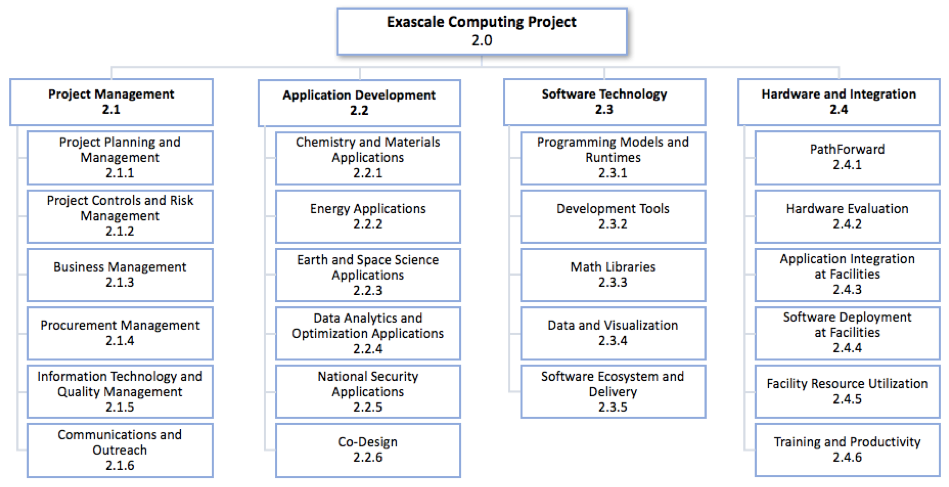
\includegraphics[width=0.9\linewidth]{ECP20}
	\caption{The ECP Work Breakdown Structure through Level 3 (L3).}
	\label{fig:ecp2}
\end{figure}

\subsection{Background}
Historically, the software used on supercomputers has come from three sources: computer system vendors, DOE laboratories, and academia. Traditionally, vendors have supplied system software:  operating system, compilers, runtime, and system-management software. The basic system software is typically augmented by software developed by the DOE HPC facilities to fill gaps or to improve management of the systems. An observation is that it is common for system software to break or not perform well when there is a jump in the scale of the system.
 
Mathematical libraries and tools for supercomputers have traditionally been developed at DOE laboratories and universities and ported to the new computer architectures when they are deployed. These math libraries and tools have been remarkably robust and have supplied some of the most impactful improvements in application performance and productivity. The challenges have been the constant adapting and tuning to rapidly changing architectures.
 
Programming paradigms and the associated programming environments that include compilers, debuggers, message passing, and associated runtimes have traditionally been developed by vendors, DOE laboratories, and universities. The same can be said for file system and storage software. An observation is that the vendor is ultimately responsible for providing a programming environment and file system with the supercomputer, but there is often a struggle to get the vendors to support software developed by others or to invest in new ideas that have few or no users yet. Another observation is that file-system software plays a key role in overall system resilience, and the difficulty of making the file-system software resilient has grown nonlinearly with the scale and complexity of the supercomputers.
 
In addition to the lessons learned from the traditional approaches, Exascale computers pose unique software challenges including the following.
\begin{itemize}
\item \textbf{Extreme parallelism:} Experience has shown that software breaks at each shift in scale. Exascale systems are predicted to have a billion-way concurrency via a combination of tasks, threads and vectorization, and more than one hundred thousand nodes. Because clock speeds have essentially stalled, the 1000-fold increase in potential performance going from Petascale to Exascale is entirely from concurrency improvements.
\item \textbf{Data movement in a deep memory hierarchy: }Data movement has been identified as a key impediment to performance and power consumption. Exascale system designs are increasing the types and layers of memory, which further challenges the software to increase data locality and reuse, while reducing data movement.
\item \textbf{Resilience:} As hardware resilience decreases due to the number of components and reduced voltage, software resilience must be developed to take up the slack and allow the Exascale system to be adaptable to component failures without the entire system crashing.  Initial concerns about resilience at the start of Exascale efforts have diminished, and the availability of non-volatile memory should dramatically improve checkpoint/restart performance.  Even so, we need to keep a focus on this issue.
\item \textbf{Power consumption:} Exascale systems have been given an aggressive power consumption goal of 20-30 MW, not much more than the power consumed by the largest systems of today. Meeting this goal will require the development of power monitoring and management software that does not exist today.
\end{itemize}
 
In addition to the software challenges imposed by the scale of Exascale computers, the following additional requirements push ECP away from the historical approaches for getting the needed software for DOE supercomputers.
\begin{itemize}
\item \textbf{2021 acceleration:} ECP has a goal of accelerating the development of the U.S. Exascale systems and enabling the first deployment by 2021. This means that the software needs to be ready sooner, and the approach of just waiting until it is ready will not work. A concerted plan that accelerates the development of the highest priority and most impactful software is needed.
\item \textbf{Productivity:} Traditional supercomputer software requires a great deal of expertise to use. ECP has a goal of making Exascale computing accessible to a wider science community than previous supercomputers have been. This requires the development of software that improves productivity and ease of use.
\item \textbf{Diversity:} There is a strong push to make software run across diverse Exascale systems. Traditionally, there has been a focus on just one new supercomputer every couple of years. ECP has a goal of enabling at least two diverse architectures, and the ECP-developed software needs to be able to run efficiently on all of them.  Some code divergence is inevitable, but careful software design, and the use of performance portability layers can minimize the amount of code targeted at a specific platform.
\item \textbf{Analytics and machine learning:} Future DOE supercomputers will need to solve emerging data science and machine learning problems in addition to the traditional modeling and simulation applications. This will require the development of scalable, parallel analytics and machine learning software that does not exist today.
\end{itemize}
 
The next section describes the approach employed by ECP ST to address the Exascale challenges.

\subsection{ECP Software Technology Approach}
ECP is taking an approach of codesign across all its principal technical areas: applications development (AD), software technology (ST), and hardware \& integration (HI). For ECP ST, this means its requirements are based on input from other areas, and there is a tight integration of the software products both within the software stack as well as with applications and the evolving hardware. 

The portfolio of projects in ECP ST is intended to address the Exascale challenges and requirements described above. We note that ECP is not developing the entire software stack for an Exascale system. For example, we expect vendors to provide the core software that comes with the system (in many cases, by leveraging ECP and other open-source efforts). Examples of vendor-provided software include operating system, file system, compilers (for C, C++, Fortran, etc.), basic math libraries, system monitoring tools, scheduler, debuggers, vendor’s performance tools, MPI (based on ECP-funded projects), OpenMP (with features from ECP-funded project), and data-centric stack components. ECP develops other, mostly higher-level software that is needed by applications and is not vendor specific. ECP-funded software activities are concerned with extreme scalability, exposing additional parallelism, unique requirements of Exascale hardware, and performance-critical components. Other software that aids in developer productivity is needed and may come from third-party open-source efforts (e.g., gdb, Valgrind).

The ST portfolio includes both ASCR and NNSA ATDM funded efforts. The MOU established between DOE-SC and NNSA has formalized this effort.  Whenever possible, ASCR and ATDM efforts are treated uniformly in ECP ST planning and assessment activities.

ST is also planning to increase integration within the ST portfolio through increased use of software components and application composition vs. monolithic application design. An important transition that ECP can accelerate is the increased development and delivery of reusable scientific software components and libraries. While math and scientific libraries have long been a successful element of the scientific software community, their use can be expanded to include other algorithms and software capabilities, so that applications can be considered more an aggregate composition of reusable components than a monolithic code that uses libraries tangentially.

To accelerate this transition, we need a greater commitment on the part of software component developers to provide reliable and portable software that users can consider to be part of the software ecosystem in much the same way users depend on MPI and compilers. At the same time, we must expect application developers to participate as clients and users of reusable components, using capabilities from components, transitioning away from (or keeping as a backup option) their own custom capabilities.

\subsubsection{Software Development Kits}\label{subsubsect:sdks}
One opportunity for a large software ecosystem project such as ECP ST is to foster increased collaboration, integration and interoperability among its funded efforts. Part of ECP ST design is the creation of software development kits (SDKs).  SDKs are collections of related software products (called packages) where coordination across package teams will improve usability and practices and foster community growth among teams that develop similar and complementary capabilities. SDKs have the following attributes:
\begin{table}
	\begin{mdframed}
\begin{enumerate}
	\item \textbf{Domain scope:} Each SDK will be composed of packages whose capabilities are within a natural functionality domain. Packages within an SDK provide similar capabilities that can enable leveraging of common requirements, design, testing and similar activities. Packages may have a tight complementary such that ready composability is valuable to the user.
	\item \textbf{Interaction models:} How packages within an SDK interact with each other. Interactions include common data infrastructure, or seamless integration of other data infrastructures; access to capabilities from one package for use in another.
	\item \textbf{Community policies:} Expectations for how package teams will conduct activities, the services they provide, software standards they follow, and other practices that can be commonly expected from a package in the SDK.
	\item \textbf{Meta-build system:} Robust tools and processes to build (from source), install and test the SDK with compatible versions of each package. This system sits on top of the existing build, install and test capabilities for each package.
	\item \textbf{Coordinated plans:} Development plans for each package will include efforts to improve SDK capabilities and lead to better integration and interoperability.
	\item \textbf{Community outreach:} Efforts to reach out to the user and client communities will include explicit focus on SDK as product suite.
\end{enumerate}
	\end{mdframed}
\caption{\label{table:sdk-attributes} Software Development Kits (SDKs) provide an aggregation of software products that have complementary or similar attributes.  ECP ST uses SDKs to better assure product interoperability and compatibility.  SDKs are also essential aggregation points for coordinated planning and testing. SDKs are an integral element of ECP ST~\cite{Heroux-SDK-Podcast}}.
\end{table}

\paragraph{ECP ST SDKs}
As part of the delivery of ECP ST capabilities, we will establish and grow a collection of SDKs. The new layer of aggregation that SDKs represent are important for improving all aspects of product development and delivery. The communities that will emerge from SDK efforts will lead to better collaboration and higher quality products. Established community policies will provide a means to grow SDKs beyond ECP to include any relevant external effort. The meta-build systems (based on Spack) will play an important role in managing the complexity of building the ECP ST software stack, by providing a new layer where versioning, consistency and build options management can be addressed at a mid-scope, below the global build of ECP ST products.
Each ECP ST L3 (five of them) has funds for an SDK project from which we will identify and establish at least one SDK effort. Fortunately, we will be able to leverage an existing SDK in the Math Libraries sub-element to inform our broader efforts. This SDK, called the xSDK, has been in existence for several years and has proven the value of an SDK approach in its domain (Figure~\ref{fig:xsdk-diagram}). 

\begin{figure}
	\centering
	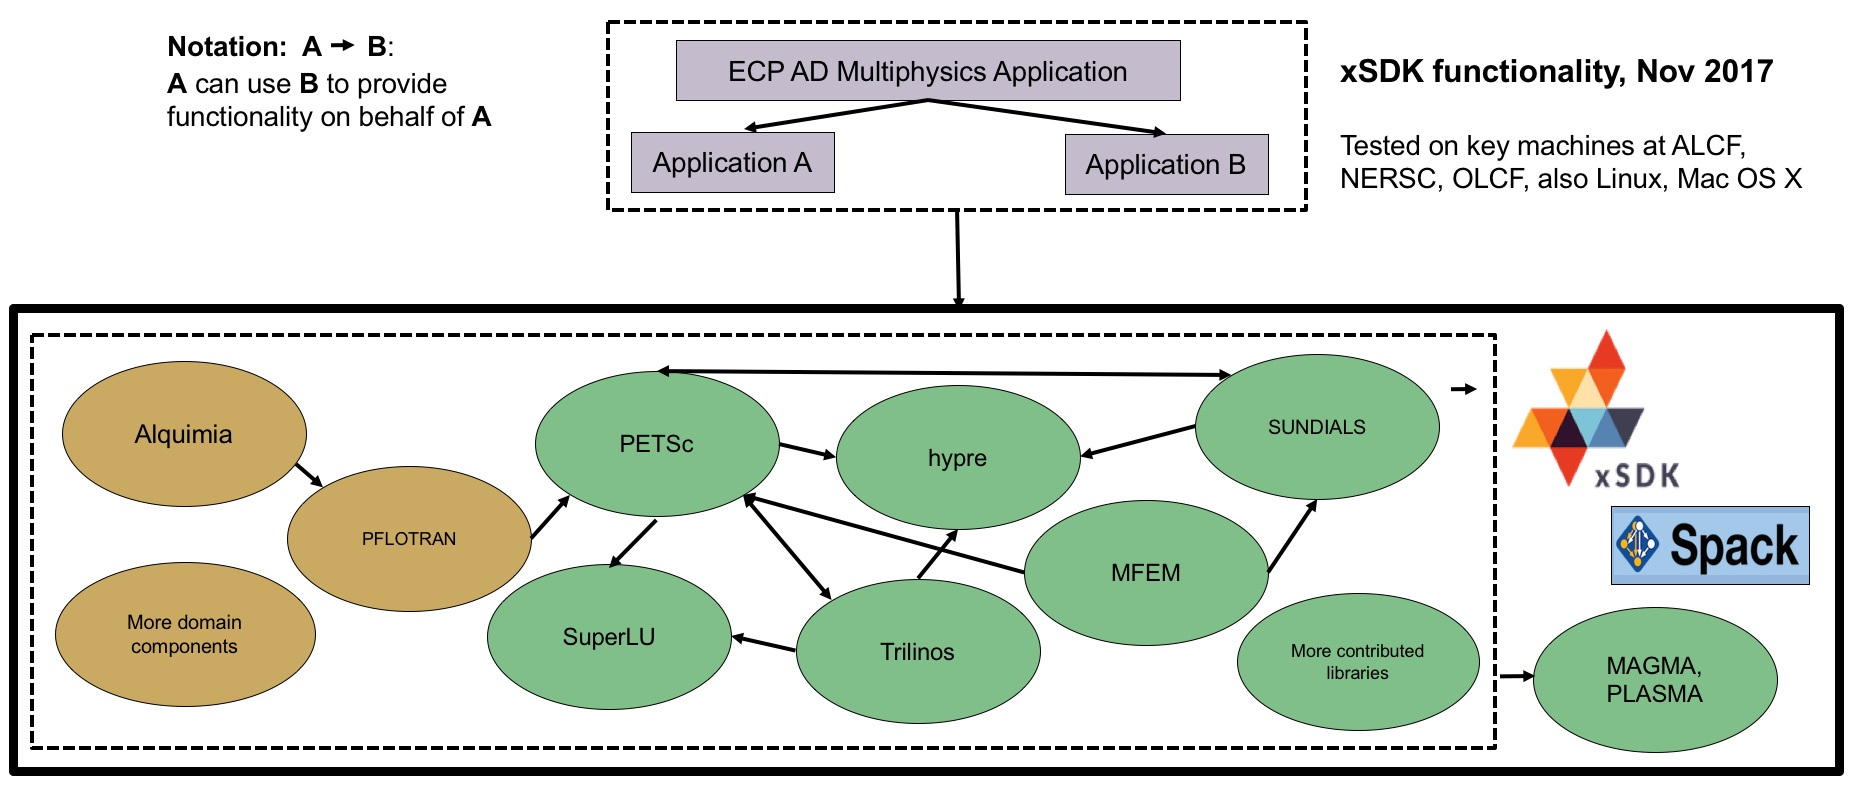
\includegraphics[width=0.9\linewidth]{xSDK-Diagram}
	\caption{The xSDK is the first SDK for ECP ST, in the Mathematical Libraries technical area~\ref{table:wbs}. The xSDK provides the collaboration environment for improving build, install and testing capabilities for member packages such as hypre, PETSc, SuperLU and Trilinos (and other products with green background). Domain components (see orange ovals) are also an important category of the ecosystem, providing leveraged investments for common components in a specific scientific software domain.  xSDK capabilities are essential for supporting the multi-physics and multi-scale application requirement that lead to combined use of xSDK libraries. Furthermore, the availability of advanced software platforms such as GitHub, Confluence, JIRA and others enable the level of collaboration needed to create an SDK from independently developed packages.}
	\label{fig:xsdk-diagram}
\end{figure}


\paragraph{The xSDK}
Initially funded by the DOE Office of Advanced Scientific Computing Research and the office of Biological and Environmental Research as part of the IDEAS Project~\cite{Bartlett:2017:XFT:3148208.3148212}, the xSDK is a collection of independent math library packages, initially the popular libraries hypre, PETSc, SuperLU and Trilinos. The xSDK was established in recognition that collaboration across independent library development efforts could have a tremendous positive impact on the math libraries capabilities provided to users, and the productivity of library developers and sustainability of library software.
Figure~\ref{fig:xsdk-diagram} illustrates the scope and interaction of xSDK packages and Figure~\ref{fig:xsdk-policies} lists the community policies that govern xSDK activities and set expectations for future xSDK members. While we recognize that xSDK experiences cannot be blindly applied to creation of new SDKs in ECP, the xSDK does provide a concrete, working example to guide ECP ST SDK efforts going forward.
\begin{figure}
	\centering
	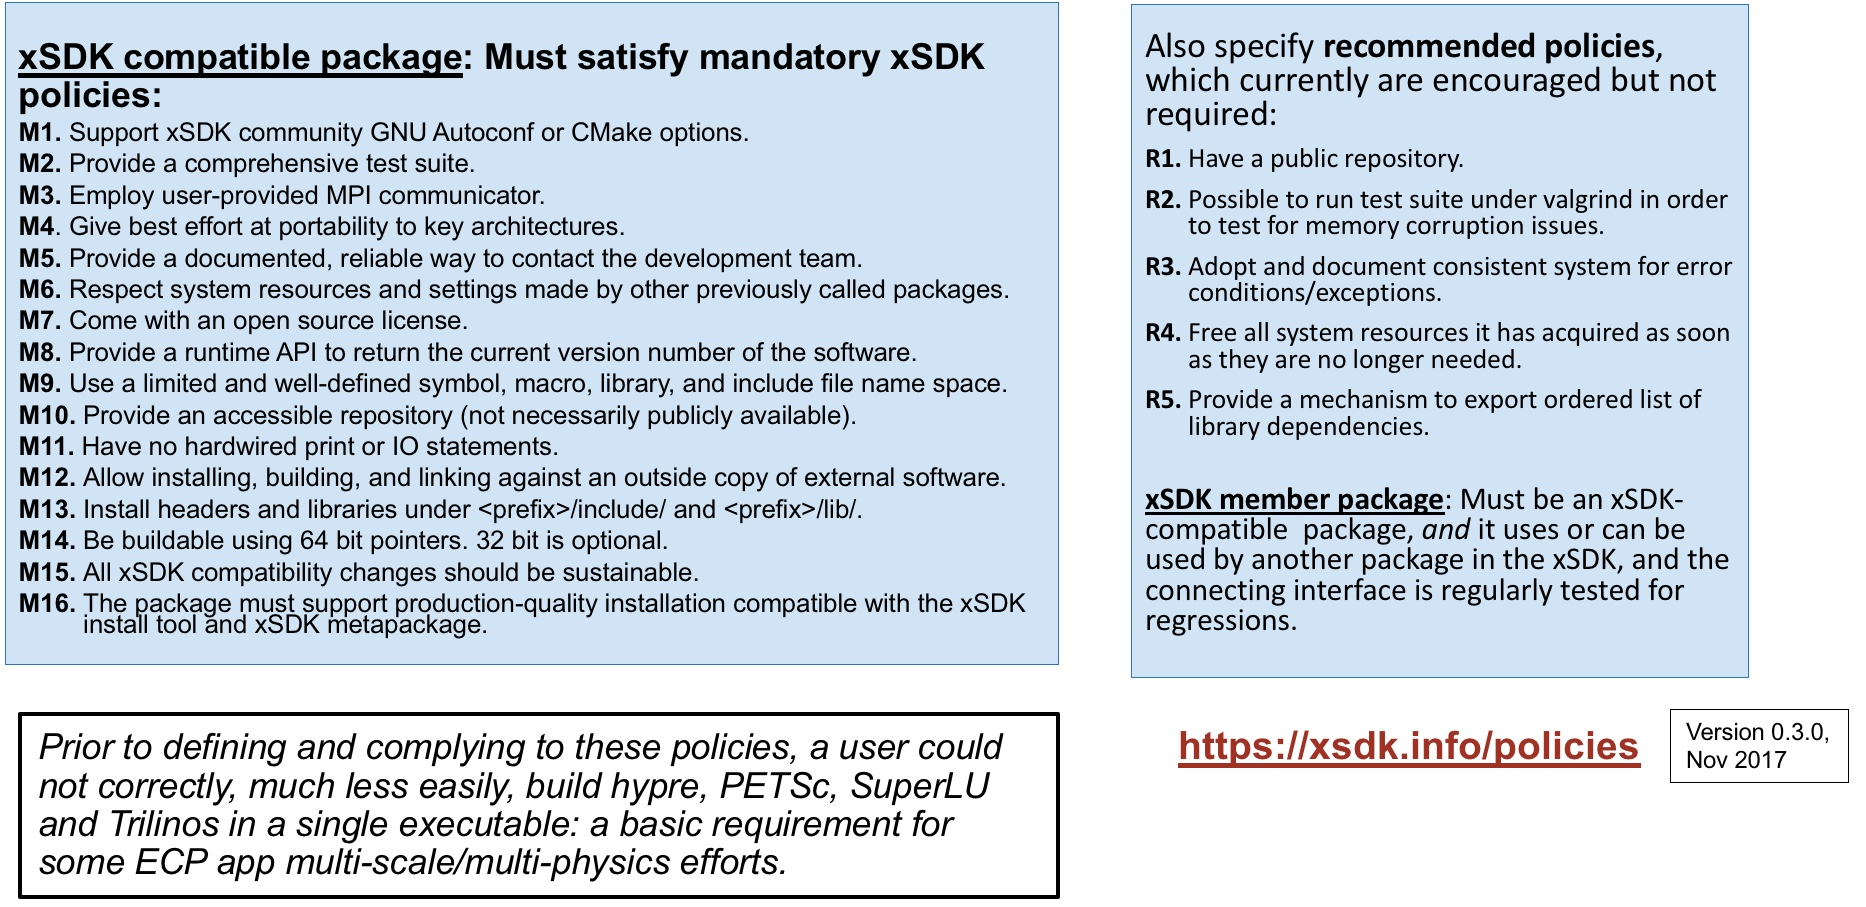
\includegraphics[width=0.9\linewidth]{xSDK-Policies}
	\caption{\textbf{xSDK Community Policies emerged from challenging and passionate discussions about essential values of the math libraries community.} Once established, these community policies represent a living statement of what it means to be part of an SDK, and are used as the criteria for welcoming future members.}
	\label{fig:xsdk-policies}
\end{figure}

\subsubsection{ECP ST Software Delivery}
An essential activity for, and the ultimate purpose of, ECP ST is the delivery of a software stack that enables productive and sustainable Exascale computing capabilities for target ECP applications and platforms, and the broader high-performance computing community. The ECP ST Software Ecosystem and Delivery sub-element (WBS 2.3.5) and the SDKs in each other sub-element provide the means by which ECP ST will deliver its capabilities.
\paragraph{ECP ST Delivery and HI Deployment}
Providing the ECP ST software stack to ECP applications requires coordination between ECP ST and ECP HI. The focus areas have a complementary arrangement where ECP ST delivers its products and ECP HI deploys them. Specifically:
\begin{itemize}
	\item ST \textbf{delivers} software.  ECP ST products are delivered directly to application teams, to vendors and to facilities.  ECP ST designs and implements products to run on DOE computing facilities platforms and make products available as source code via GitHub, GitLab or some other accessible repository.
	\item HI facilitates efforts to \textbf{deploy} ST (and other) software on Facilities platforms by installing it where users expect to find it. This could be in /usr/local/bin or similar directory, or available via “module load”.
\end{itemize}
Separating the concerns of delivery and deployment is essential because these activities require different skill sets. Furthermore, ECP ST delivers its capabilities to an audience that is beyond the scope of specific Facilities’ platforms. This broad scope is essential for the sustainability of ECP ST products, expanding the user and developer communities needed for vitality. In addition, ECP HI, the computer system vendors and other parties provide deployable software outside the scope of ECP ST, therefore having the critical mass of skills to deploy the entire software stack.

\paragraph{ECP ST Delivery Strategy}
ECP ST delivers it software products as source code, primarily in repositories found on GitHub, Gitlab installations or similar platforms. Clients such as ECP HI, OpenHPC and application developers with direct repository access then take the source and build, install and test our software. The delivery strategy is outlined in Figure~\ref{fig:softwarestack}.  

Users access ECP ST products using these basic mechanisms (see Figure~\ref{fig:productsoverview} for deliverable statistics):
\begin{itemize}
	\item \textbf{Build from source code:} The vast majority of ECP ST products reach at least some of their user base via direct source code download from the product repository.  In some cases, the user will download a single compressed file containing product source, then expand the file to expose the collection of source and build files.  Increasingly, users will fork a new copy of an online repository.  After obtaining the source, the user executes a configuration process that detects local compilers and libraries and then builds the product.  This kind of access can represent a barrier for some users, since the user needs to build the product and can encounter a variety of challenges in that process, such as an incompatible compiler or a missing third-party library that must first be installed.  However, building from source can be a preferred approach for users who want control over compiler settings, or want to adapt how the product is used, for example, turning on or off optional features, or creating adaptations that extend product capabilities.  For example, large library frameworks such as PETSc and Trilinos have many tunable features that can benefit from the user building from source code.  Furthermore, these frameworks support user-defined functional extensions that are easier to support when the user builds the product from source.  ECP ST is leveraging and contributing to the development of Spack~\cite{gamblin+:sc15}.  Via meta-data stored in a Spack \textit{package} defined for each product, Spack leverages a product's native build environment, along with knowledge about its dependencies, to build the product and dependencies from source.  Spack plays a central role in ECP ST software development and delivery processes by supporting turnkey builds of the ECP ST software stack for the purposes of continuous integration testing, installation and seamless multi-product builds.
	\item \textbf{DOE computing facilities:} Each DOE computing facility (ALCF, OLCF, NERSC, LLNL and ACES [LANL/SNL]) provides pre-built versions of 17 to 20 ECP ST products (although the exact mix of products varies somewhat at each site).  Many of these products are what users would consider to be part of the core system capabilities, including compilers, e.g., Flang (Section~\ref{subsubsect:flang}) and LLVM (Section~\ref{subsubsect:sollve}), and parallel programming environments such as MPICH (Section~\ref{subsubsect:mpich}), OpenMPI (Section~\ref{subsubsect:openmpi}) and OpenMP (Section~\ref{subsubsect:bolt}).  Development tools such as PAPI (Section~\ref{subsubsect:exapapi}) and TAU (Section~\ref{subsubsect:tau}) are often part of this suite, if not already included in the vendor stack. Math and data libraries such as PETSc (Section~\ref{subsubsect:petsc}), Trilinos (Section~\ref{subsubsect:trilinos}), HDF5 (Section~\ref{subsubsect:exahdf5}) and others are also available in some facilities software installations.  We anticipate and hope for increased collaboration with facilities via the ECP Hardware \& Integration (HI) Focus Area.  We are also encouraged by multi-lab efforts such as the Tri-Lab Operating System Stack (TOSS)~\cite{TOSS} that are focused on improving uniformity of software stacks across facilities.
	\item \textbf{Vendor stacks:} Computer system vendors leverage DOE investments in compilers, tools and libraries.  Of particular note are the wide use of MPICH(Section~\ref{subsubsect:mpich}) as software base for most HPC vendor MPI implementations and the requirements, analysis, design and prototyping that ECP ST teams provide.  Section~\ref{subsection:external-contributions} describes some of these efforts.
	\item \textbf{Binary distributions:} Approximately 10 ECP ST products are available via binary distributions such as common Linux distributions, in particular via OpenHPC\cite{OpenHPC}.  ECP ST intends to foster growth of availability via binary distributions as an important way to increase the size of the user community and improve product sustainability via this broader user base.
\end{itemize}

\begin{figure}
	\centering
	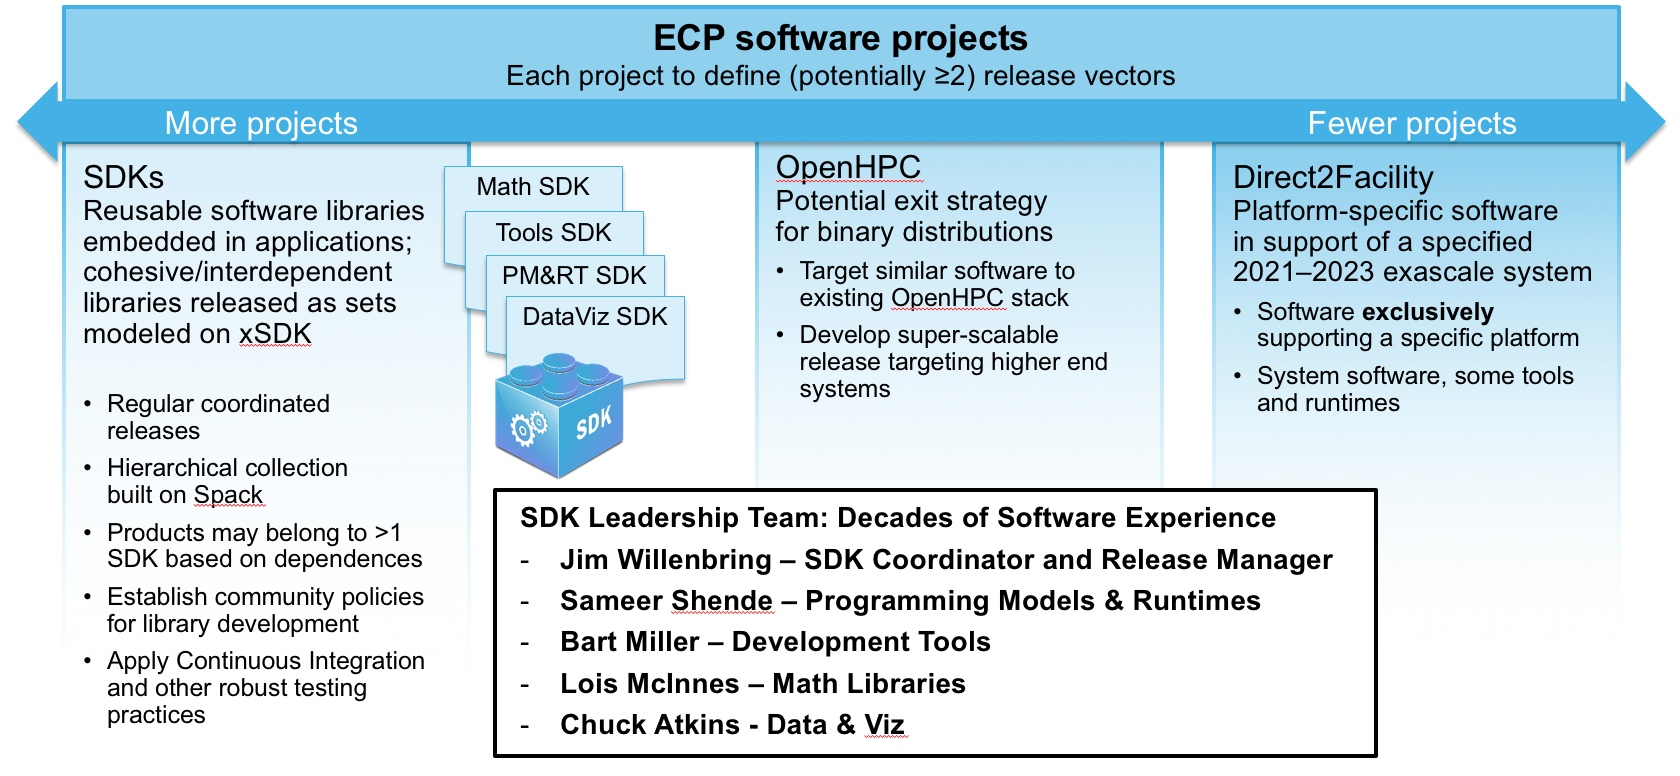
\includegraphics[width=0.9\linewidth]{SoftwareStack}
	\caption{\textbf{The ECP ST software stack is delivered to the user community through several channels.} Key channels are via source code, increasing using SDKs, direct to Facilities in collaboration with ECP HI, via binary distributions, in particular the OpenHPC project and via HPC vendors.  The SDK leadership team includes  ECP ST team members with decades of experience delivering scientific software products.}
	\label{fig:softwarestack}
\end{figure}

\subsection{ECP ST Project Restructuring}\label{subsect:ProjectRestructuring}

The initial organization of ECP ST was based on discussions that occurred over several years of Exascale planning within DOE, especially the DOE Office of Advanced Scientific Computing Research (ASCR).  Figure~\ref{fig:ecpstv1} shows the conceptual diagram of this first phase.  The 66 ECP ST projects were mapped into 8 technical areas, in some cases arbitrating where a project should go based on its primary type of work, even if other work was present in the project.  In November 2017, ECP ST was reorganized into 5 technical areas, primarily through merging a few smaller areas, and the number of projects was reduced to 56 (presently 55 due to further merging in \ecosystem).  Figure

\begin{table}
\begin{tabular}{|L{1in}|L{1in}|L{1.0in}|L{2.5in}|}\hline
\textbf{WBS} & \textbf{Role/Area} & \textbf{Leader} & \textbf{Transition} \\\hline
1.3 & ECP ST Director & Rajeev Thakur & Renumbered to 2.3.  Thakur left director role, continues as lead of 2.3.1 \pmr. Mike Heroux new director. \\\hline
1.3 & ECP ST Deputy Director & Pat McCormick & McCormick left deputy role, continued as PI of 2.3.1.08 Legion project. Jonathan Carter new deputy director.\\\hline
1.3.1 & Programming Models \& Runtimes & Rajeev Thakur& Renumbered to 2.3.1, renamed to \pmr, otherwise unchanged. \\\hline
1.3.2 & Tools & Jeffrey Vetter
& Renumbered to 2.3.2, renamed to \tools, otherwise unchanged. \\\hline
1.3.3 & Math/Scientific Libs & Mike Heroux & New leader Lois Curfman McInnes, renamed Mathematical Libraries, new number 2.3.3. \\\hline
1.3.4 & Data Management \& Workflows & Rob Ross & Combined with 1.3.5 to create 2.3.4. Jim Ahrens leader. \\\hline
1.3.5 & Data Analytics \& Visualization & Jim Ahrens
& Combined with 1.3.4 to create 2.3.4. Jim Ahrens leader.\\\hline
1.3.6 & System Software & Martin Schulz& Combined with 1.3.7 and 1.3.8 into 2.3.5. Rob Neely leader.\\\hline
1.3.7 & Resilience & Al Geist & Combined with 1.3.6 and 1.3.8 into 2.3.5. Rob Neely leader. \\\hline
1.3.8 & Integration & Rob Neely & 
Combined with 1.3.6 and 1.3.7 into 2.3.5. Rob Neely leader. \\\hline
\end{tabular}
	\caption{\label{fig:wbs-transition}ECP ST technical areas were reduced from 8 to 5 in November 2017.  This figure shows how areas were remapped and merged.  In addition, the ECP ST Director and Deputy Director changed from Rajeev Thakur (who continues as the \pmr\ lead) and Pat McCormick to Mike Heroux and Jonathan Carter, respectively.}
\end{table}

\begin{figure}
\begin{mdframed}
\begin{itemize}
\item Phase 1: 66 total projects
\begin{itemize}
\item 35 projects funded by the DOE Office of Science that were selected in late 2016 via an RFI and RFP process, considering prioritized requirements of applications and DOE facilities. 
These projects started work in January–March 2017 depending on when the contracts were awarded.
\item 31 ongoing DOE NNSA funded projects that are part of the Advanced Technology Development and Mitigation (ATDM) program. The ATDM program started in FY14.  These projects are focused on longer term research to address the shift in computing technology to extreme, heterogeneous architectures and to advance the capabilities of NNSA simulation codes.
\end{itemize}
\item Phase 2: 56 total projects
(now 55 after further merging in 2.3.5)
\begin{itemize}
\item 41 ASCR-funded projects.  Added  2 \ecosystem\ projects and 4 SDK projects.
\item 15 ATDM projects: Combined the previous 31 ATDM projects into one project per technical area per lab.  ATDM projects are generally more vertically integrated and would not perfectly mapped to any proposed ECP ST technical structure.  Minimizing the number of ATDM projects within the ECP WBS structure reduces complexity of ATDM to ECP coordination and gives ATDM flexibility in revising its porfolio without disruption to the ECP-ATDM mapping.
\end{itemize}
\end{itemize}
\end{mdframed}

\caption{\label{fig:project-remapping}Project remapping summary from Phase 1 (through November 2017) to Phase 2 (After November 2017)}
\end{figure}


\begin{figure}
	\centering
	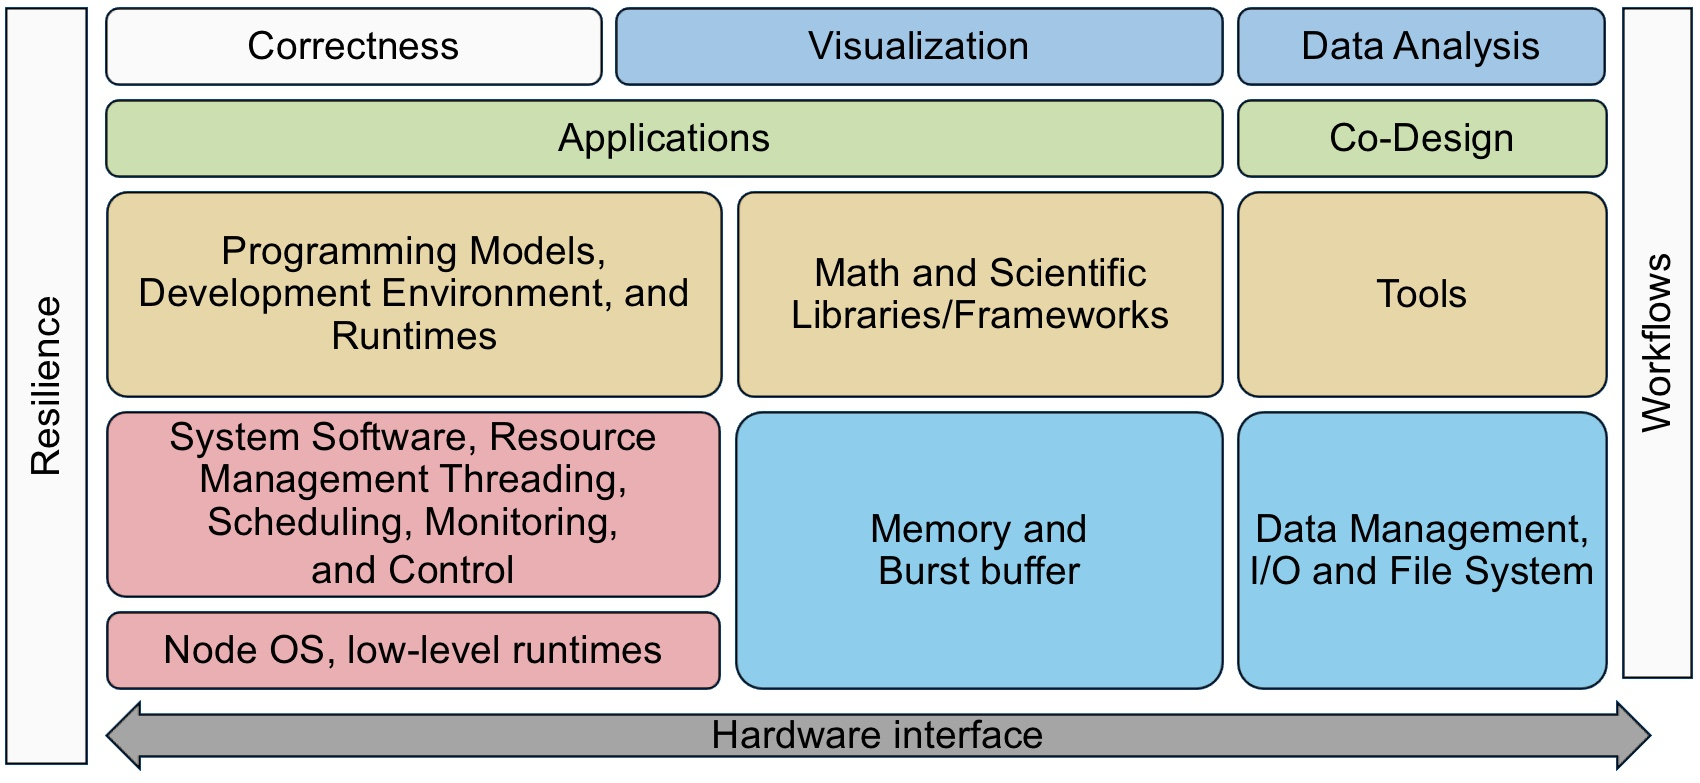
\includegraphics[width=0.9\linewidth]{ECPSTV1}
	\caption{ECP ST before November 2017 reorganization.  This conceptually layout emerged from several years of Exascale planning, conducted primarily within the DOE Office of Advanced Scientific Computing Research (ASCR).  After a significant restructuring of ECP that removed much of the facilities activities and reduced the project timeline from 10 to seven years, and a growing awareness of what risks had diminished, this diagram no longer represented ECP ST efforts accurately.}
	\label{fig:ecpstv1}
\end{figure}
\begin{figure}
	\centering
	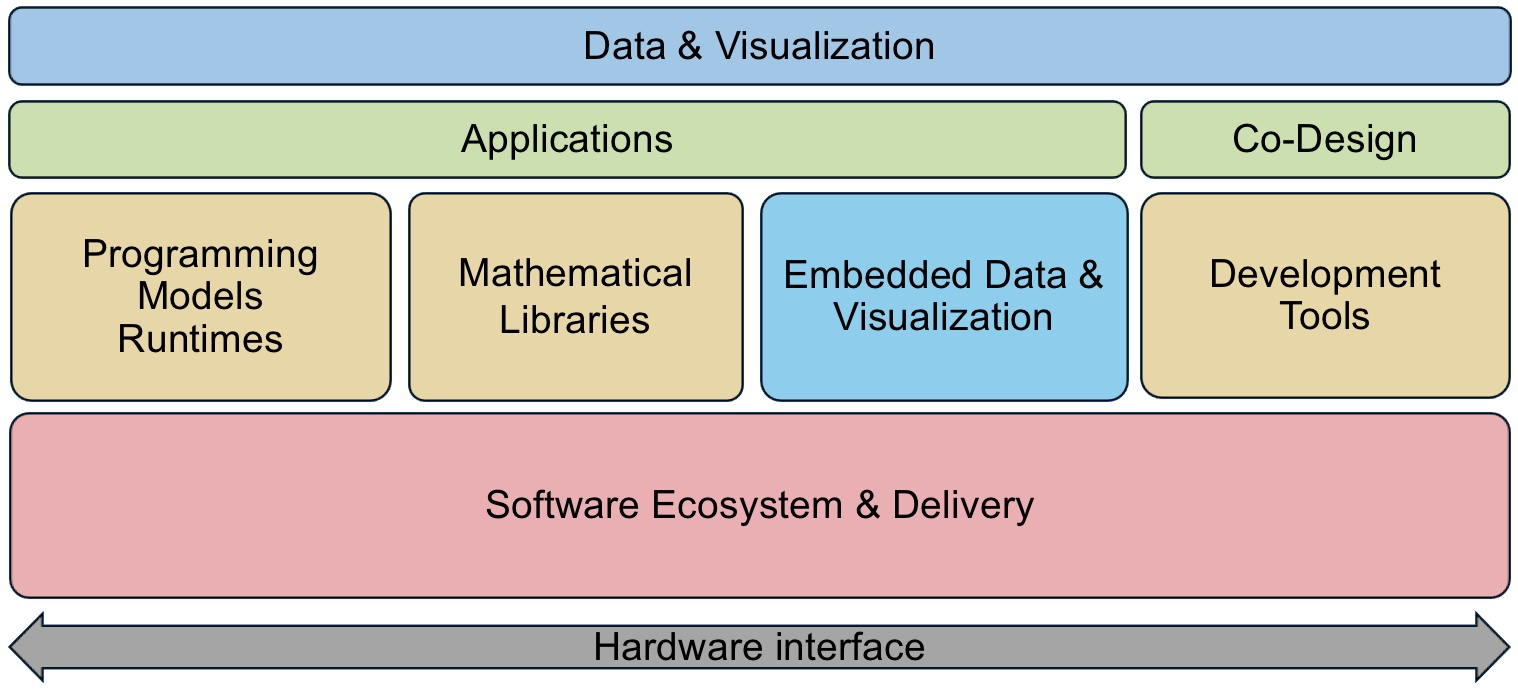
\includegraphics[width=0.9\linewidth]{ECPSTV2}
	\caption{ECP ST after November 2017 reorganization.  This diagram more accurately reflects the priorities and efforts of ECP ST given the new ECP project scope and the demands that we foresee.}
	\label{fig:expstv2}
\end{figure}
\begin{figure}
	\centering
	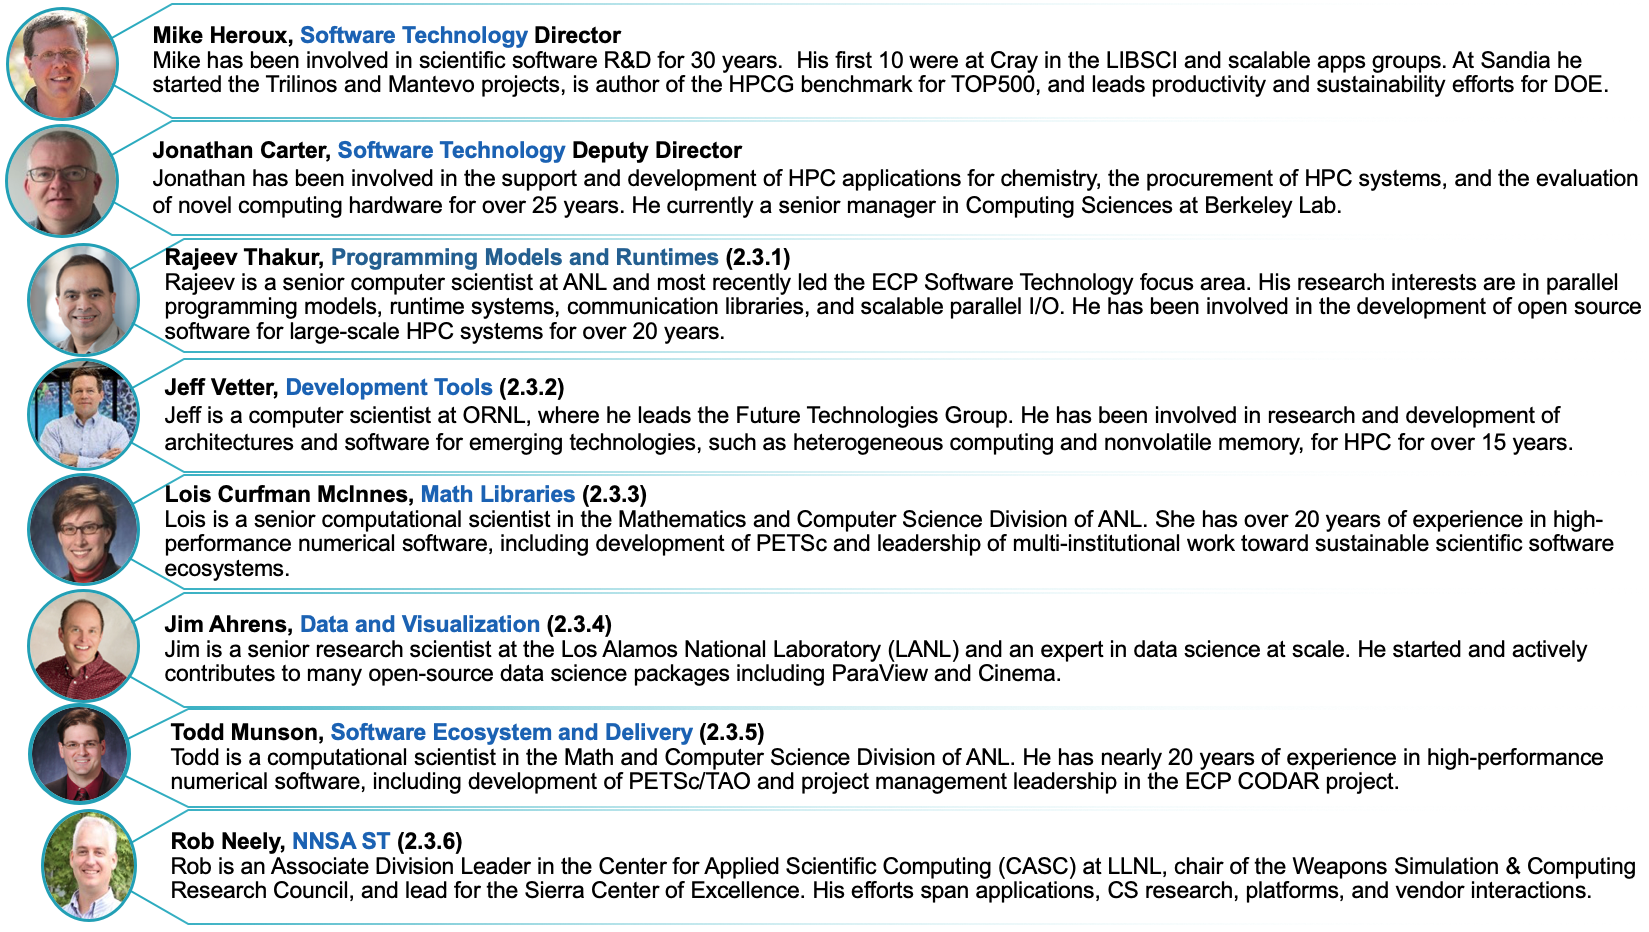
\includegraphics[width=0.9\linewidth]{ECP-ST-Leads}
	\caption{ECP ST Leadership Team as of November 2017.}
	\label{fig:ecpstleads}
\end{figure}

\subsection{New Project Efforts}
ECP ST has initiated four newly-funded efforts as a result of findings in our September 2017 Gap Analysis~\cite{Thakur2017GapAnalysis}.  We anticipate several additional efforts in the coming months in order to mitigate some of the higher risks we have identified in programming environments and data management.  We will report this second phase of additions in the next version of this report.

\subsubsection{FFTs}\label{subsubsect:ffts}
ECP ST has initiated two new efforts in Fast Fourier Transforms (FFTs).  FFTs provide an essential mathematical tool to many application areas.  From the very beginning of HPC, vendors have provided optimized FFT libraries for their users.  The advent of FFTW~\cite{FFTW05}, a tunable high-performance library with a well-designed interface, enabled a \textit{de facto} standardization of FFT interfaces, and an effective source base for vendor libraries, which adapted FFTW source for their platforms.

There is some concern in the community that FFTW is no longer actively developed, nor well prepared for emerging platforms.  Furthermore, FFTW's strong copylefting license (which forces its users to make their own software open source in the same way) has always been a challenge to users.  While vendors are still committed to providing optimized FFT libraries, whether or not FFTW is available, we believe it is prudent to explore a new software stack and have funded a short-term project to explore this possibility.  The new library will also explore problem formulations that could significantly reduce the computational cost of FFTs.  This new effort, called FFTX, will be led by Lawrence Berkeley National Lab, under the existing math libraries project (Section~\ref{subsubsect:strumpack}).

A second FFT project will address a consensus opportunity to provide a sustainable 3D FFT library built from established but \textit{ad hoc} software tools that have traditionally been part of application codes, but not extracted as independent, supported libraries.  These 3D FFTs rely on third-party 1D FFTs, either from FFTW or from vendor libraries.

The goal of this second project, FFT-ECP, led by the University of Tennessee and integrated into one of its existing projects (Section~\ref{subsubsect:slate}) is to:
\begin{itemize}
\item Collect existing FFT capabilities recently made available from ECP application teams (LAMMPS/fftMPI and HACC/SWFFT). 
\item Assess gaps and make available as a sustainable math library.
\item Explore opportunities to build 3D FFT libraries on vendor 1D and 2D kernels, especially leveraging on-node concurrency from 2D and batched 1D formulations.
\item Focus on capabilities for Exascale platforms.
\item Emphasize leverage of vendor capabilities and addressing vendor deficiencies over creation of new and independent software stack.
\end{itemize}

This effort, while not addressing the concerns about FFTW directly, is essential to providing a new and sustainable FFT software stack that leverages the large investment by the broader HPC community in FFT software.  The payoff from this effort is almost guaranteed.  Also, should the FFTX project also go forward, it will provide an FFTW-compatible interface that would allow FFT-ECP to use FFTX as one option, in addition to external FFT libraries.

\subsubsection{LLNL Math Libraries}\label{subsubsect:llnl-math-libs}
When ECP ST started, some important capabilities were not part of the original portfolio, even though their engagement is essential for ECP application success.  This is true of the LLNL math library \textit{hypre}~\cite{hypre}.  This library is widely used to provide scalable multigrid preconditioners across several ECP applications.  Funding to support adaptation of \textit{hypre}  in preparation for Exascale platforms at science lab facilities, e.g., Argonne, and for ECP science applications was not part of the original ECP ST portfolio.  We have added funding for this effort, starting in June 2018.  In addition, we provided new funding for another LLNL math library, MFEM~\cite{mfem:homepage}, so that the MFEM team can participate in SDK efforts for math libraries.